\documentclass[12pt,a4paper]{article}
\usepackage{graphicx}
\usepackage{array}
\usepackage{longtable}
\usepackage{geometry}
\usepackage{float}
\usepackage{tabularx}
\geometry{margin=1in}



\begin{document}

% ── Title Page ───────────────────────────────────────────────
\begin{titlepage}
  \centering
  \vspace*{6.5cm}
  {\LARGE \textbf{Network Intrusion Detection System} \\[0.5em]
    \textbf{Powered by Machine Learning}}\\[2cm]
  {\large Phase 1: Analysis and Design}\\[2cm]
  {\large Amira BOUAFIF \& Hajer JEMAA}\\[0.5cm]
  \vfill
  {\large 2025-2026}\\[1cm]
\end{titlepage}

\section*{Introduction}

With the increasing number of cyberattacks targeting modern networks, detecting malicious activity has become an essential task for organizations. Traditional security systems often struggle to keep up with the volume and complexity of current network traffic. For this reason, machine learning techniques are increasingly used to improve intrusion detection.

This project focuses on the design and analysis of a Network Intrusion Detection System (NIDS). In this phase, we define the technical architecture, select the dataset, choose appropriate algorithms and the evaluation metrics. We also present the use case, class and architecture diagrams.
\section{Technical Stack}
\begin{itemize}
  \item \textbf{AI Engine:} Python (TensorFlow, PyTorch, scikit-learn, XGBoost).
  \item \textbf{AI microservice:} FastAPI (lightweight, high-performance API framework).
  \item \textbf{Backend:} Spring Boot (robust REST APIs, scalable, enterprise-ready).
  \item \textbf{Database:} MySQL.
  \item \textbf{Frontend:} React (custom dashboard for monitoring and analytics).
  \item \textbf{Authentication:} Spring Security + JWT.
  \item \textbf{Real-time:} Server-Sent Events (SSE).
  \item \textbf{Model Serialization:} Joblib (.pkl).
  \item \textbf{Deployment:} Docker containers; optional Kubernetes for scalability.
\end{itemize}

\section{Dataset Choice}
\begin{table}[h!]
  \begin{center}
    \begin{tabularx}{\textwidth}{|l|X|}
      \hline
      \textbf{Property} & \textbf{Value}                                                  \\
      \hline
      Dataset           & CIC-IDS2017                                                     \\
      \hline
      Source            & Canadian Institute for Cybersecurity                            \\
      \hline
      Format            & CSV (pre-extracted features)                                    \\
      \hline
      Size              & $\approx$ 2.8M records across 8 CSV files                       \\
      \hline
      Feature count     & 78 features per flow record                                     \\
      \hline
      Attack types      & DoS, DDos, Probe, Brute Force, Web Attack, Botnet, Infiltration \\
      \hline
    \end{tabularx}
    \caption{Dataset properties}
    \label{tab1}
  \end{center}
\end{table}

\textbf{Justification }
\begin{itemize}
  \item Comprehensive labeled dataset with multiple attack types (DoS, DDoS, Brute Force, etc.)
  \item Widely used benchmark, realistic traffic, suitable for ML/DL experiments.
\end{itemize}


\section{Algorithms Choice}
\begin{itemize}
  \item \textbf{Machine Learning:} Decision Tree (baseline), XGBoost (main model).
  \item \textbf{Anomaly Detection (future work):} Autoencoders, hybrid chained/parallel approaches.
\end{itemize}


\vskip0.5cm
\noindent\textbf{Justification for the XGBoost model:}
\vskip0.5cm
\begin{itemize}
  \item High accuracy on CIC-IDS2017 benchmark
  \item Fast inference time suitable for near real-time detection
  \item Low memory footprint for API deployment via FastAPI
  \item No GPU requirement as it is deployable on standard hardware
\end{itemize}

\section{Metrics}

\begin{table}[h!]
  \begin{center}
    \begin{tabularx}{\textwidth}{|l|l|l|X|}
      \hline
      \textbf{Metric}     & \textbf{Target} & \textbf{Priority} & \textbf{Justification}                          \\
      \hline
      Accuracy            & $\geq 98\%$     & High              & Standard benchmark on CIC-IDS2017               \\
      \hline
      F1-Score (macro)    & $\geq 0.95$     & High              & Handles class imbalance across attack types     \\
      \hline
      False Positive Rate & $\leq 2\%$      & Critical          & Too many false alerts causes alert fatigue      \\
      \hline
      False Negative Rate & $\leq 1\%$      & Critical          & Missed attacks represent a security breach      \\
      \hline
      Inference Time      & $\leq 200ms$    & High              & Near real-time requirement\\
      \hline
    \end{tabularx}
    \caption{Target Metrics }
    \label{tab2}
  \end{center}
\end{table}

\section{AI / Detection Engine}

\begin{itemize}
  \item Data preprocessing pipeline (cleaning, normalization, encoding)
  \item XGBoost training and evaluation
  \item Model serialization (.pkl file via Joblib)
  \item FastAPI microservice exposing \texttt{POST /predict} endpoint
  \item Input: CIC-IDS2017 feature vector (78 features)
  \item Output: \texttt{\{ label: String, confidence: float \}}
\end{itemize}

\section{Backend}

\begin{itemize}
  \item REST API for alert management (CRUD)
  \item REST API for network flow submission and storage
  \item Integration with FastAPI via HTTP client (WebClient)
  \item Alert, NetworkFlow and AuditLog persistence in MySQL
  \item Auto-generation of weekly reports
  \item Server-Sent Events (SSE) endpoint for real-time alert push
  \item JWT authentication (login / logout)
  \item Role-based access control (\texttt{ADMIN} / \texttt{IT\_MANAGER})
\end{itemize}

\section{Frontend}

\begin{itemize}
  \item Login page
  \item Dashboard : real-time alert counter, attack type distribution
        chart, network flow volume over time
  \item Statistics Summary page : aggregated security metrics
  \item Alerts List page : paginated and searchable
  \item Alert Detail page : full flow data and status management
        (\texttt{REVIEWED} / \texttt{DISMISSED})
  \item Reports page : view auto-generated reports and export
  \item Real-time updates via Server-Sent Events (SSE)
\end{itemize}

\section{Modeling}
\subsection{Use Case Diagram}
\vskip1cm
\begin{figure}[H]
  \centering
  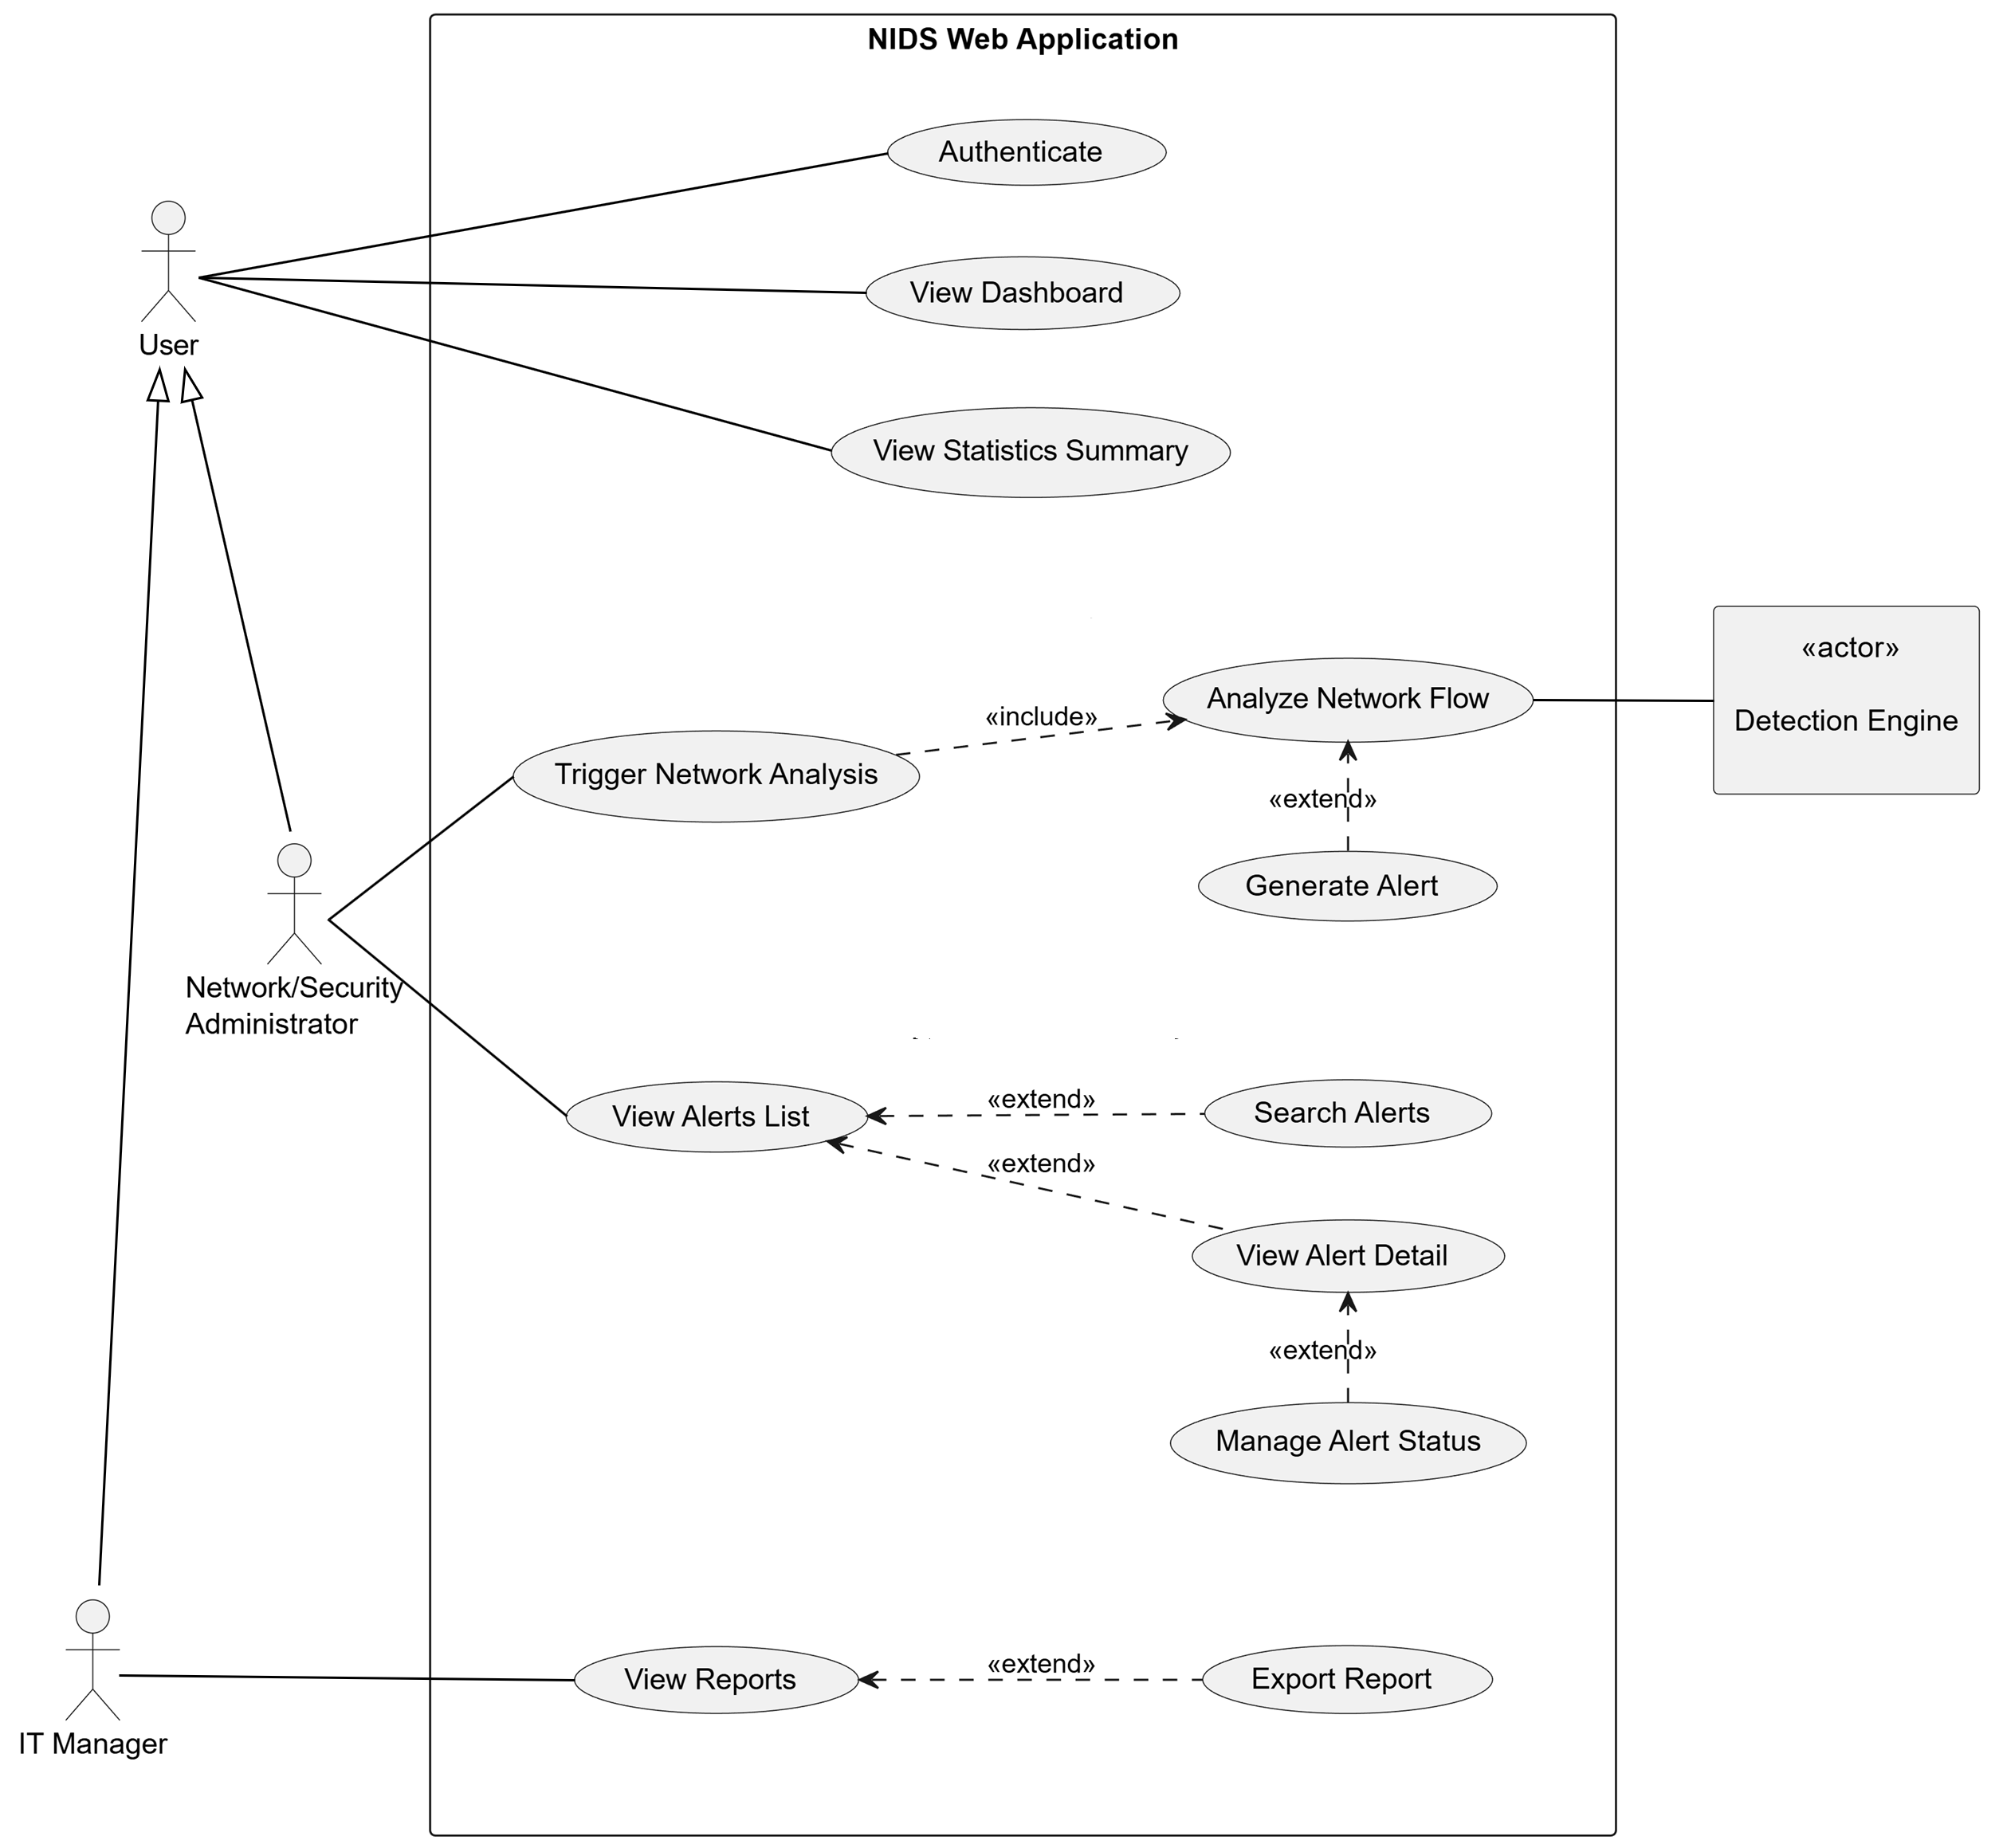
\includegraphics[width=1\columnwidth]{diagrams/use-case.png}
  \caption{Use Case Diagram}
  \label{fig:Usecase-Diagram}
\end{figure}

\subsection{Class Diagram}

\begin{figure}[H]
  \centering
  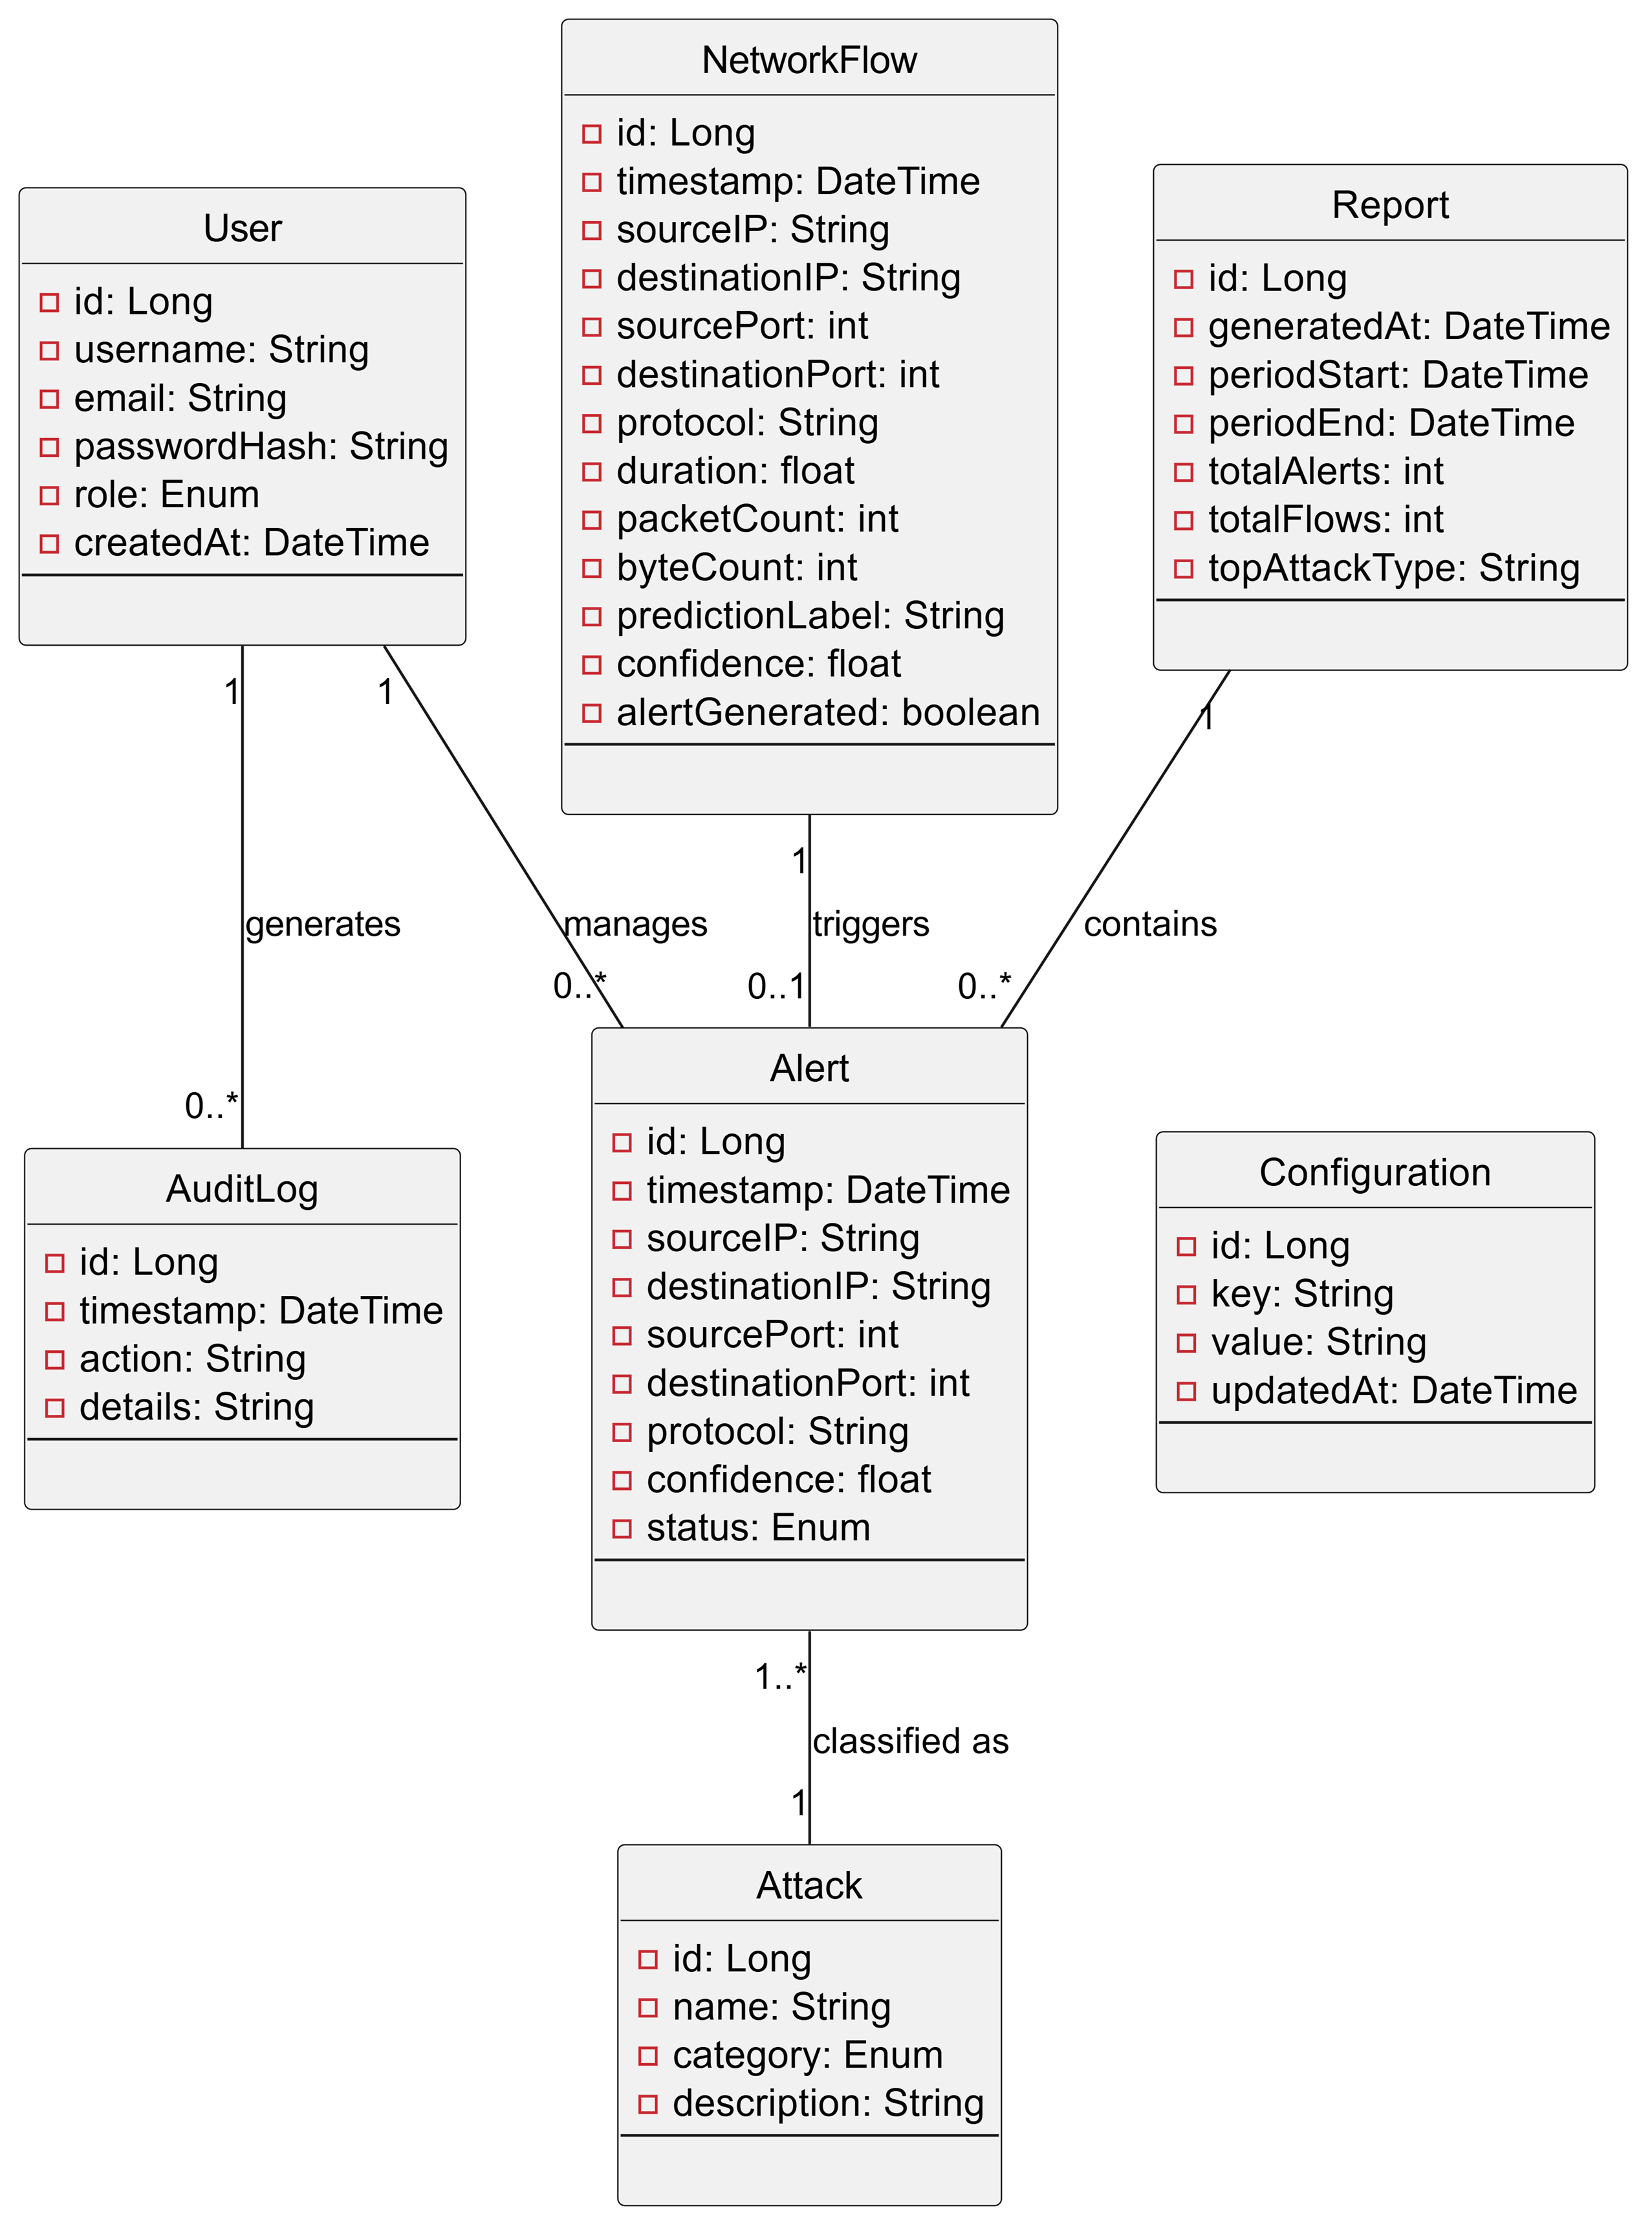
\includegraphics[width=1\columnwidth]{diagrams/class.png}
  \caption{Class Diagram}
  \label{fig:Class-Diagram}
\end{figure}

\subsection{Architecture Diagram}
\vskip1cm
\begin{figure}[H]
  \centering
  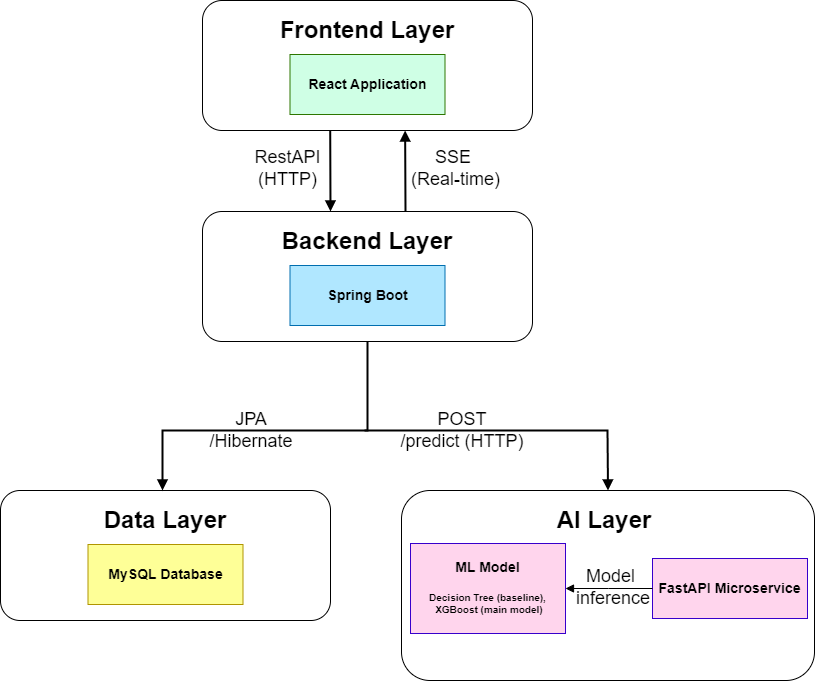
\includegraphics[width=1\columnwidth]{diagrams/archie.png}
  \caption{Architecture Diagram}
  \label{fig:Architecture-Diagram}
\end{figure}
\newpage
\section{Product Backlog}
\begin{longtable}{|p{3cm}|p{6cm}|p{6cm}|}
  \hline
  \textbf{Weeks} & \textbf{Tasks}                              & \textbf{Deliverables}                                                                                                                  \\
  \hline
  1--5           & Data understanding + preparation            & Preprocessing scripts, dataset report                                                                                                  \\
  \hline
  6--10           & Baseline ML models (Decision Tree, XGBoost) & Trained models, evaluation metrics                                                                                                     \\
  \hline
  11--12          & Backend + Frontend integration              & Spring Boot APIs, React dashboard                                                                                                      \\
  \hline
  13--14         & Testing + reporting                         & Validation, documentation, and reporting End-to-end demo, detailed logs, visualizations, automated security report, final presentation \\
  \hline
\end{longtable}

\section*{Conclusion}
This phase established the foundation of the project by defining the system architecture, selecting the dataset, and identifying the machine learning models that will be used for intrusion detection. The proposed solution combines a machine learning detection engine with a web-based monitoring platform, allowing security alerts to be analyzed in real time. The next stages of the project will focus on the data understanding and preprocessing.
\end{document}